\section{Offline Simulation and Results}
The process used for the offline simulation is the same as Chapter \ref{A8_cahp}. The feeder components use the same data as chapter \ref{A8_cahp} as well. Fig. \ref{fig:OFFLINE1_NM_ES} shows the offline simulation result for the energy storage using a NYISO based RTP. The $r_{es}(1)$ and $r_{es}(2)$ values are 5 cents/kWh and 7 cents/kWh. The other properties of the energy storage are the same as table \ref{tab:es}. The solid red line is ES1 SOC, the dashed blue line is ES2 SOC and the dotted black line is the RTP.
As it can be seen from fig. \ref{fig:OFFLINE1_NM_ES} they behave as expected. Both ES1 and ES2 charge during low price points and discharge during high price points. Fig. \ref{fig:GEN_COST_CURVE} shows the cost curve for the generator. The A and B values for the generator are 0.001\$ and 0.0001\$. Fig. \ref{fig:OFFLINE1_NM_Gen} shows the response of the energy provided by the generator and the grid. The solid red line is the energy supplied by the generator. The dashed blue line is the energy supplied by the grid and the dotted black line is RTP. It can be seen that during high price point the generator supplies energy. There is also a significant dip in the grid energy supply during the high price points. This signifies that the algorithm is behaving as expected.
Fig. \ref{fig:OFF_7_day_NYISO_ES} and fig. \ref{fig:OFF_7_day_NYISO_GEN} shows seven day test runs for the scenarios described in fig. \ref{fig:OFFLINE1_NM_ES} and fig. \ref{fig:OFFLINE1_NM_Gen} respectively. In the previous scenario, a NYISO based RTP was used for simulation. The algorithm has also been simulated using a PG\&E Time of Use (TOU) price based RTP as well. Fig. \ref{fig:OFF_7_day_PGNE_ES} shows the seven day simulation results for the energy storages, and fig. \ref{fig:OFF_7_day_PGNE_GEN} shows the seven day simulation results for the generator and grid.
\begin{figure}[!ht]
\centering
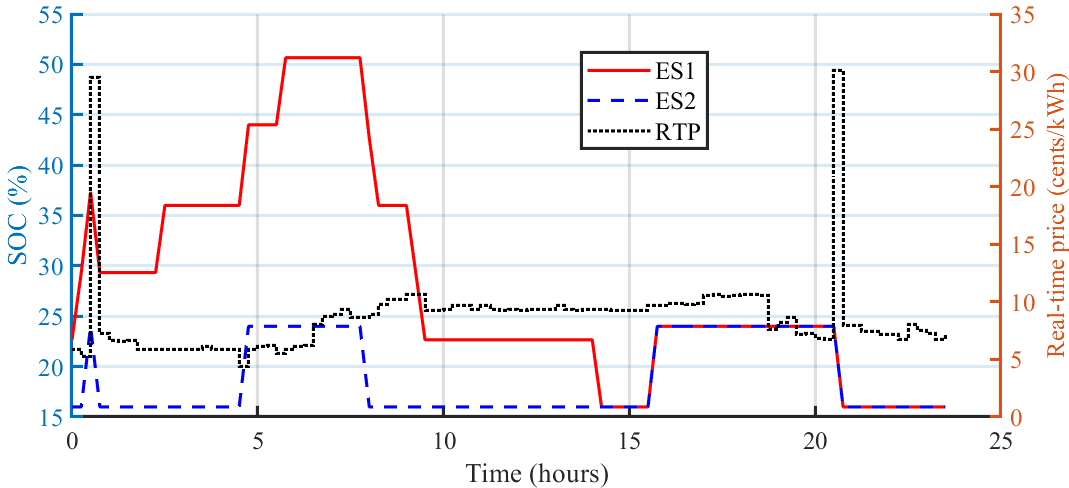
\includegraphics[width = \linewidth]{figs/A82/OFFLINE1_NM_ES.png}
\caption{Offline one day ES results with NYISO based RTP}
\label{fig:OFFLINE1_NM_ES}
\end{figure}

\begin{figure}[!ht]
\centering
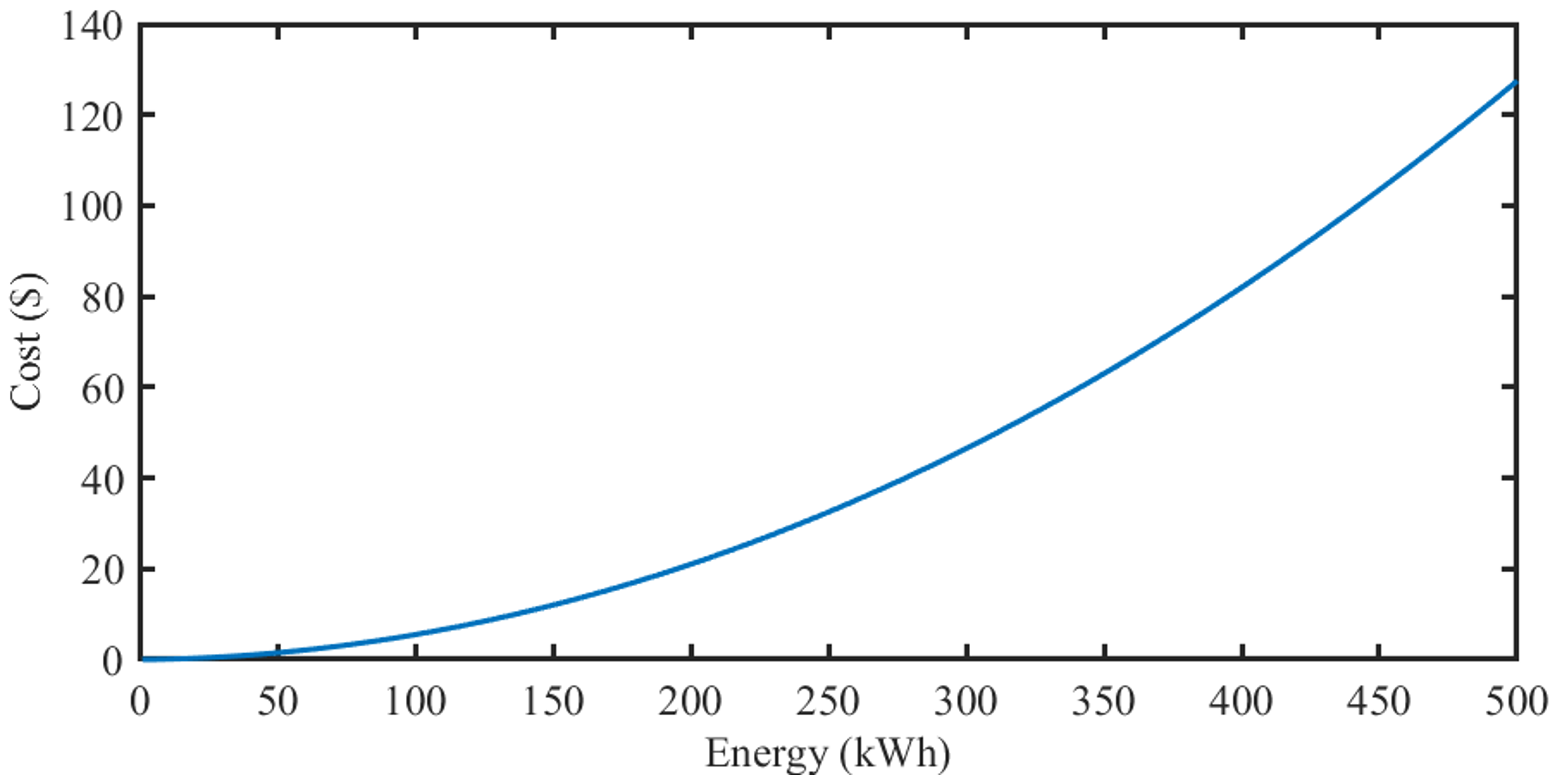
\includegraphics[width = \linewidth]{figs/A82/GEN_COST_CURVE.png}
\caption{Cost curve of the generator}
\label{fig:GEN_COST_CURVE}
\end{figure}

\begin{figure}[!ht]
\centering
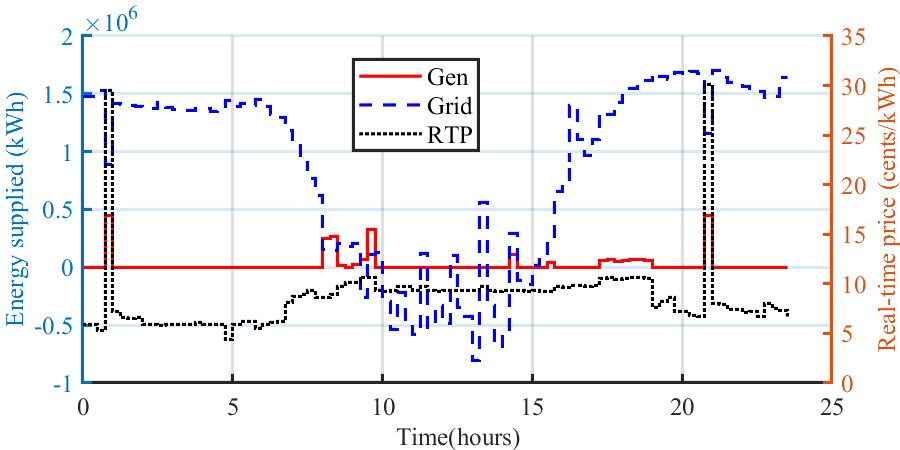
\includegraphics[width = \linewidth]{figs/A82/OFFLINE1_NM_GEN.png}
\caption{Offline one day gen and grid results with NYISO based RTP}
\label{fig:OFFLINE1_NM_Gen}
\end{figure}

\begin{figure}[!ht]
\centering
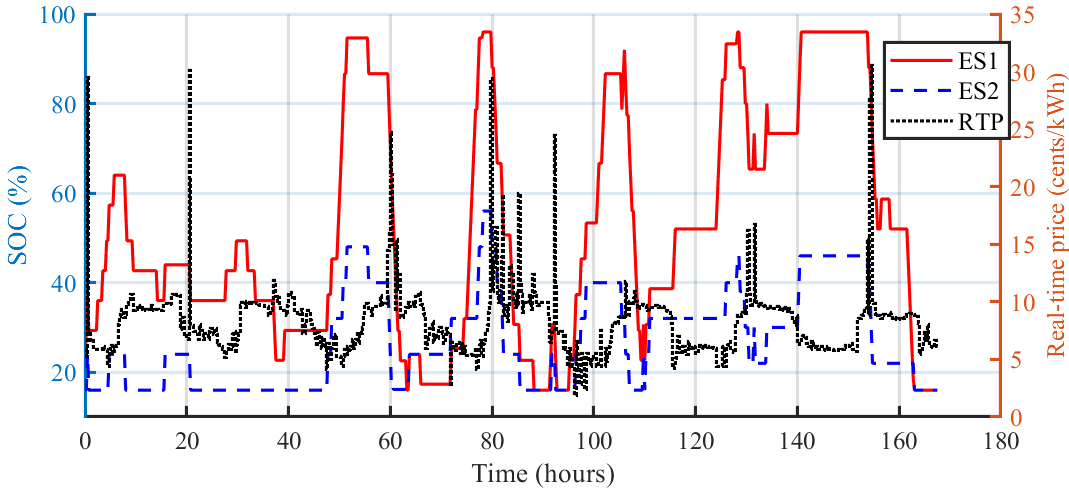
\includegraphics[width = \linewidth]{figs/A82/OFF_7_day_NYISO_ES.png}
\caption{Offline ES results with NYISO based RTP for seven days}
\label{fig:OFF_7_day_NYISO_ES}
\end{figure}


\begin{figure}[!ht]
\centering
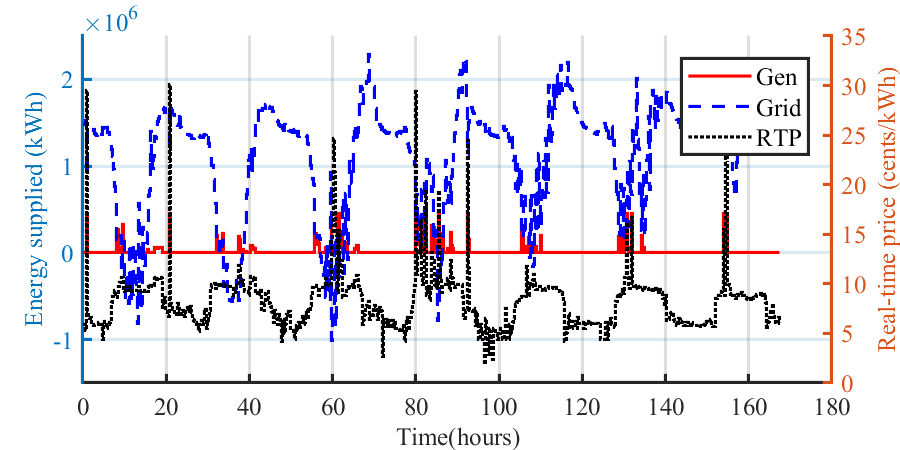
\includegraphics[width = \linewidth]{figs/A82/OFF_7_day_NYISO_GEN.png}
\caption{Offline gen and grid results with NYISO based RTP for seven days}
\label{fig:OFF_7_day_NYISO_GEN}
\end{figure}

\begin{figure}[!ht]
\centering
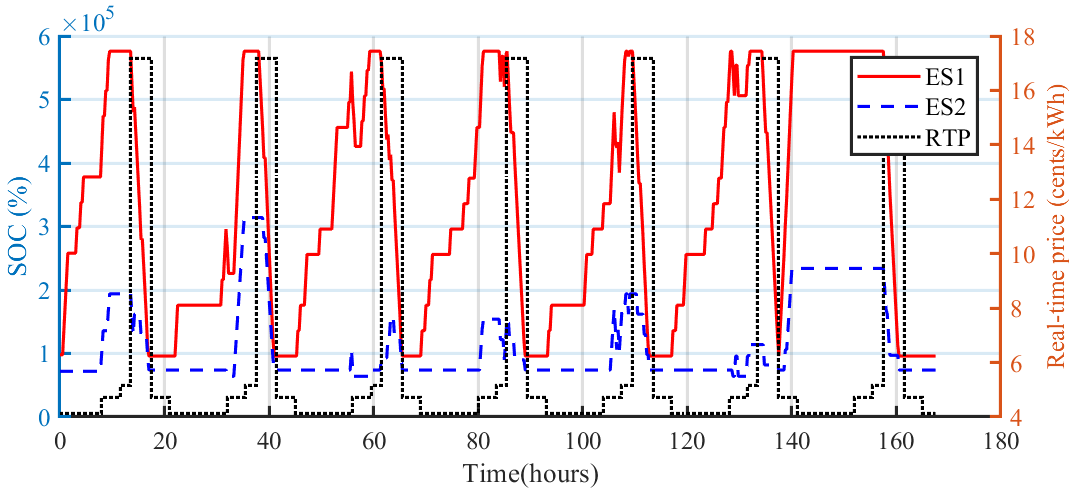
\includegraphics[width = \linewidth]{figs/A82/OFF_7_day_PGNE_ES.png}
\caption{Offline ES results with PG\&E based RTP for seven days}
\label{fig:OFF_7_day_PGNE_ES}
\end{figure}


\begin{figure}[!ht]
\centering
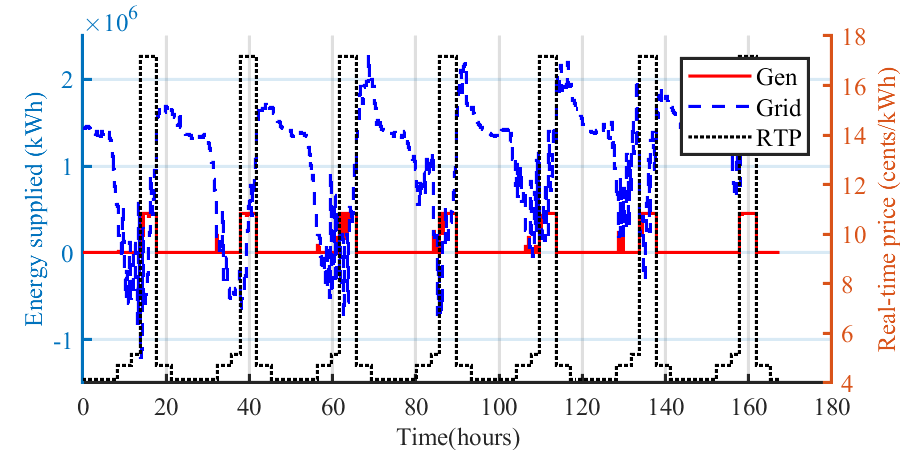
\includegraphics[width = \linewidth]{figs/A82/OFF_7_day_PGNE_GEN.png}
\caption{Offline gen and grid results with PG\&E based RTP for seven days}
\label{fig:OFF_7_day_PGNE_GEN}
\end{figure}

To validate the efficiency of the algorithm the previously mentioned NYISO and PG\&E RTP scenarios have been tested against two test cases.

Case1 is PSO based approach. The performance of the seven day test results shown in fig. \ref{fig:OFF_7_day_NYISO_ES}, fig. \ref{fig:OFF_7_day_NYISO_GEN}, fig. \ref{fig:OFF_7_day_PGNE_ES}, and fig. \ref{fig:OFF_7_day_PGNE_GEN} have been first compared against a PSO based approach. The PSO based approach used PSO to solve a modified version of (\ref{eq:multi_all_in1_sys}). The PSO problem formulation is as follows:
minimize:
\begin{multline}
\label{eq:multi_all_in1_PSO}
    ( P_{grid}*rtp + |(P_{es}(1)*r_{es}(1)| + |(P_{es}(2)*r_{es}(2)| \\ + A*P_{Gen}^2 + B*P_{Gen} )*\Delta T
\end{multline}
Subject to:

$(\delta_1 - \delta_2)/X_{12} = P_{Grid}$

$(\delta_2 - \delta_1)/X_{12}+ (\delta_2 - \delta_3/X_{23} = P_{L2}$

$(\delta_3 - \delta_2)/X_{23}+(\delta_3 - \delta_4)/X_{34}+(\delta_3 - \delta_7)/X_{37} = P_{L3}$

$(\delta_4 - \delta_3)/X_{34}+(\delta_4 - \delta_4)/X_{45}+(\delta_4 - \delta_6)/X_{46}=P_{L4} -$

$P_{PV1} - P_{es}(1) - P_{PV}(1)$

$(\delta_5 - \delta_4)/X_{45} = P_{L5}-P_{Gen}$

$(\delta_6 - \delta_4)/X_{46} = P_{L6}$

$(\delta_7 - \delta_3)/X_{37} + (\delta_7 - \delta_8)/X_{78}  = P_{L7}$

$(\delta_8 - \delta_7)/X_{78} + (\delta_8 - \delta_9)/X_{89}  = P_{L8} - P_{es}(2) - P_{PV}(2)$

$(\delta_9 - \delta_8)/X_{89} = -P_{PV}(3)$

$0 \leq P_{Gen} \leq \overline{P_{Gen}}$

$\underline{ES(1)} \leq ES_{current}(1)+(P_{es}(1)*\Delta T) \leq \overline{ES(1)}$

$\underline{ES(2)} \leq ES_{current}(2)+(P_{es}(2)*\Delta T) \leq \overline{ES(2)}$

$\underline{P_{ES}(1)} \leq P_{es}(1) \leq \overline{P_{ES}(1)}$

$\underline{P_{ES}(2)} \leq P_{es}(2) \leq \overline{P_{ES}(2)}$\\


Equation (\ref{eq:multi_all_in1_PSO}) is solved using the matlab 'particleswarm' solver \cite{MW_PSO}. The PSO based case performed much slower than the graph search based approach in this case. The comparison between all the cases are presented in table \ref{tab:Cost_MULTI}. It can be observed from the table that the PSO based approach is 4.3\% to 4.5\% less efficient compared to the graph search solution case. It can also be seen that where the graph search based solution takes an average of around 211 S to 234 s on average to finish calculation for one time-step (15  minutes), and the PSO based approach takes around 521 S to 462 s on average to finish the same calculation. In this case, it is evident that the graph search based solution provides a more cost efficient result in less time.

Case2 is GA based approach. In the GA based approach, the genetic algorithm solver available in matlab global minimum solver \cite{MW_GA} is used to solve (\ref{eq:multi_all_in1_PSO}) for each time-step. The cost and time taken for calculation for the GA case is shown in Table \ref{tab:Cost_MULTI}. It can be seen from the table that the GA based approach is 3.1\% to 3.2\% less efficient compared to the graph search solution case. The GA based case also takes around 921 S to 913 s on average to finish the calculations. This is a lot more time required to do the calculations and it is over the allotted time-step of 900s to finish the calculation. Compared to the graph search based approach the GA based approach is a lot less time efficient in this case. In fact, taking over 900 s to complete calculations for 900 s long time steps makes the approach not suitable for real-time calculation on the field.

\begin{table}
\caption{Seven day comparison between graph search, PSO, and GA based approach}
\label{tab:Cost_MULTI}
\begin{tabular}{l|l|l|}
\cline{2-3}
                                                        & NYISO                   & PG\&E                \\ \hline
\multicolumn{1}{|l|}{PSO}                               & Cost = 481,102.47185 \$ & Cost = 578,430.01 \$ \\ 
\multicolumn{1}{|l|}{}                                  & Time = 521 s            & Time = 462 s         \\ \hline
\multicolumn{1}{|l|}{GA}                                & Cost = 476,028.52 \$    & Cost =570,680.70 \$  \\ 
\multicolumn{1}{|l|}{}                                  & Time = 921 s            & Time = 913 s         \\ \hline
\multicolumn{1}{|l|}{Graph search}                      & Cost=461,267.95 \$      & Cost=553,521.54 \$   \\ 
\multicolumn{1}{|c|}{}                                  & Time = 234 s          & Time = 211 s       \\ \hline
\multicolumn{1}{|l|}{Cost saving wrt PSO (\%)} & 4.30\%                  & 4.50\%               \\ \hline
\multicolumn{1}{|l|}{Cost saving wrt GA (\%)}  & 3.20\%                  & 3.10\%               \\ \hline
\end{tabular}
\end{table}

\subsection{Effects of Discretization and Time-Step}
In the tests performed before, the ES SOCs were discretized using steps of 2\% and the time step was set to 15 minutes. This part shows the effects of changing discretization and time-steps on both time and cost. Table \ref{tab:MULTI_TIME_DELTA} shows the effect changing discretization and time-step. It shows seven day offline test results using the NYISO price profile for 2\%, 3\%, and 5\% discretization and 15 minute, 30 minute, and 60 minute time steps. The results clearly show that increasing time-step or discretization values result in less time to get a solution but it also results in a higher cost.
\begin{table}[htb]
\caption{Effects of discretization and time-step on the algorithm performance}
\centering
\label{tab:MULTI_TIME_DELTA}
\begin{tabular}{|l|l|l|l|}
\hline
Discretization & 15 minute & 30 minute & 60 minute \\ \hline
2\% ES capacity & \begin{tabular}[c]{@{}l@{}}Cost: \$461,267.95
\\ Time: 234.1
s\end{tabular} & \begin{tabular}[c]{@{}l@{}}Cost: \$480,179.93
\\ Time: 131.1s\end{tabular} & \begin{tabular}[c]{@{}l@{}}Cost: \$507,070.01
\\ Time: 49.16s\end{tabular} \\ \hline

3\% ES capacity & \begin{tabular}[c]{@{}l@{}}Cost: \$475,105.98
\\ Time: 159.18s\end{tabular} & \begin{tabular}[c]{@{}l@{}}Cost: \$494,585.33
\\ Time: 89.15s\end{tabular} & \begin{tabular}[c]{@{}l@{}}Cost: \$522,282.11
\\ Time: 33.42s\end{tabular} \\ \hline

5\% ES capacity & \begin{tabular}[c]{@{}l@{}}Cost: \$483,408.81
\\ Time: 56.18s\end{tabular} & \begin{tabular}[c]{@{}l@{}}Cost: \$503,228.57
\\ Time: 31.46s\end{tabular} & \begin{tabular}[c]{@{}l@{}}Cost: \$531,409.373
\\ Time: 11.79s\end{tabular} \\ \hline
\end{tabular}
\end{table}

\subsection{Starting With Different SOC}
Similar to the previous chapter the ES1 and ES2 are started from a SOC of 50\% and 24\%. The responses of ES1 and ES2 are shown in  fig. \ref{fig:OFF_DIFF_SOC_ES12}. It can be seen that similar to the single ES example shown in the previous chapter, ES1 ans ES2 are taking into account the extra starting energy to decide the charging and discharging actions. Fig. \ref{fig:OFF_DIFF_SOC_GRID_GEN} shows the response of the generator and grid. It can be seen that the generator response does not depend on the starting position of the ES. It has the same response as fig. \ref{fig:OFFLINE1_NM_Gen}.

\begin{figure}[!ht]
\centering
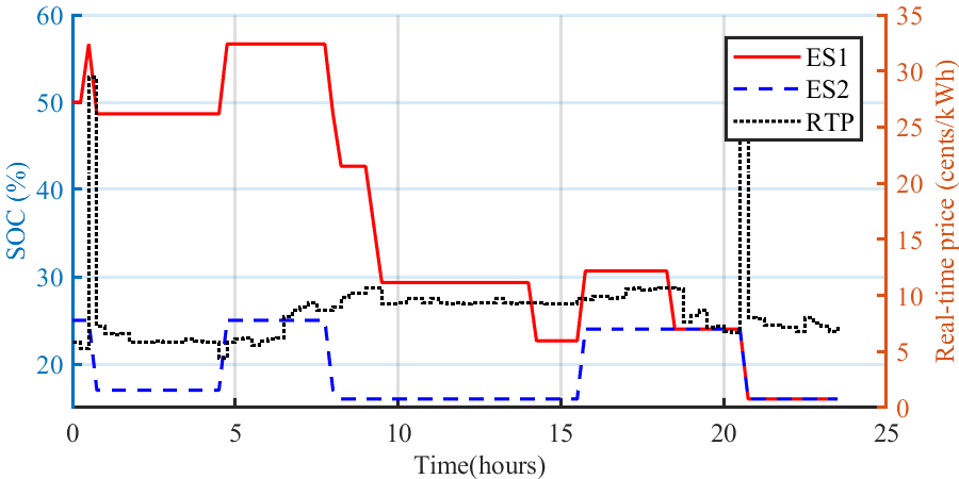
\includegraphics[width = \linewidth]{figs/A82/OFF_DIFF_SOC_ES12.png}
\caption{Starting from different SOC, ES1 and ES2 responses.}
\label{fig:OFF_DIFF_SOC_ES12}
\end{figure}

\begin{figure}[!ht]
\centering
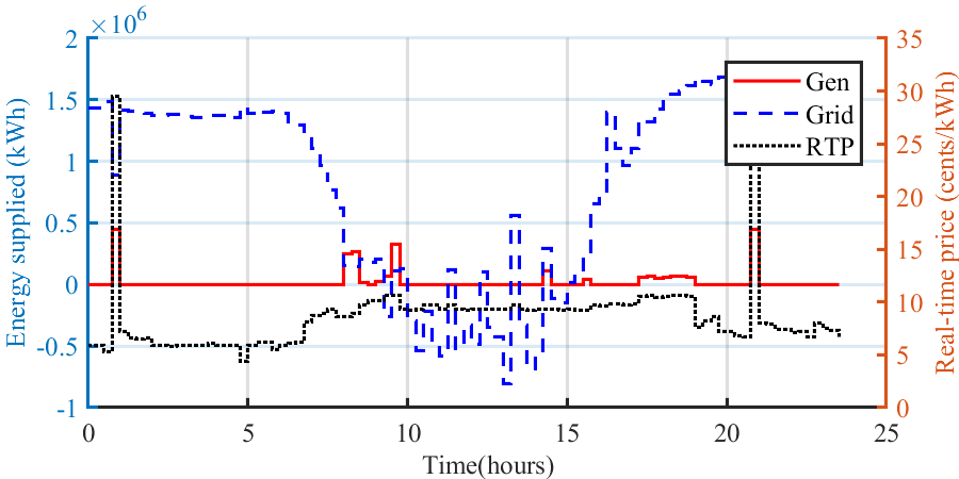
\includegraphics[width = \linewidth]{figs/A82/OFF_DIFF_SOC_GRID_GEN.png}
\caption{Starting from different SOC, generator and grid responses.}
\label{fig:OFF_DIFF_SOC_GRID_GEN}
\end{figure}
